% This template was originally by R. Jacob Vogelstein
% Updated on March 1, 2010 by Noah J. Cowan


\documentclass[12pt,oneside,final]{thesis}

\usepackage[superscript]{cite}
\usepackage{amsmath,amsfonts}
\usepackage{graphicx}
\graphicspath{{./figs/}}
\usepackage{fixltx2e}
\usepackage{array}
% wrapfig is fragile: use sparingly
\usepackage{wrapfig} 
%\usepackage{times}  % Use this for ugly fonts

\usepackage{upgreek}
\usepackage{hyperref}
\usepackage{setspace}

\usepackage{booktabs}
\usepackage{multirow}
\usepackage{longtable}
\usepackage[font=singlespacing, labelfont=bf]{caption}
%\usepackage{CV}

\usepackage{enumitem}
\newlist{inlinelist}{enumerate*}{1}
\setlist*[inlinelist,1]{%
  label=(\arabic*),
}

\usepackage{fancyhdr}    % Use nice looking headers along with the required footer page numbers   
%\usepackage[hypertex]{hyperref}

%Define the header/footer style
\pagestyle{fancy}
\fancyhf{}
\setlength{\headheight}{15pt}
\lhead{\leftmark}
\cfoot{\thepage}
\renewcommand{\headrulewidth}{0pt}
\fancypagestyle{plain}{% Redefine ``plain'' style for chapter boundaries
\fancyhf{} % clear all header and footer fields
\fancyfoot[C]{\thepage} % except the center
\renewcommand{\headrulewidth}{0pt}
\renewcommand{\footrulewidth}{0pt}}

%\tolerance=10000

%\makeglossary % enable the glossary

\begin{document}

\title{Modulo7 : A full stack Music Information Retrieval and Querying Engine using Music Theoretic Principles}
\author{Arunav Sanyal}
\degreemonth{December}
\degreeyear{2015} 
\thesis
\masterscience
\copyrightnotice


% add your chapters, best way is to have separate TeX files for each chapter
%% FRONTMATTER
\begin{frontmatter}

% generate title
\maketitle

\begin{abstract}

\noindent Music Information Retrieval (MIR) is an interdisciplinary science of extracting non trivial information and statistics from music data sources. In today's digital age, music is stored in a variety of digitized formats - e.g midi, musicxml, mp3, digitized sheet music etc. Music Information Retrieval Software aim at extracting features from one or more of these source. MIR research helps in solving problems like automatic music classification, recommendation engine design etc. Users can then query the acquired statistics to acquire relevant information. \\\\
The author proposes and implements a new Music Information Retrieval and Query Engine called Modulo7. Unlike other MIR software which deal with low level audio features, Modulo7 operates on the principles of music theory and a symbolic representation of music. Modulo7 is a full stack deployment, with server components that parse various sources of music data into its own efficient internal representation and a client component that allows consumers to query the system with sql like queries which satisfies certain music theory criteria (and as a consequence Modulo7 has a custom relational algebra with its basic building blocks based on music theory). 

\vspace{1cm}

\noindent Primary Reader: Dr David Yarowsky\\
Secondary Reader: Dr Yanif Ahmad

\end{abstract}

\begin{acknowledgment}

I would like to thank Dr David Yarowsky for giving me the opportunity to work on this project. His detailed insights have immensely helpful to me to power through my work. I would like to thank Dr Yanif Ahmad for his crucial help in the systems aspects of my query engine and the implementation of the server side components. 

\end{acknowledgment}

\begin{dedication}
 
This thesis is dedicated to my family and to all the music lovers in the world. 

\end{dedication}

% generate table of contents
\tableofcontents

\end{frontmatter}

\chapter{Introduction}
\label{sec:intro}

\noindent Why does a person like a particular song? What are the inherent aspects of a song that pleases a person's musical taste? Is it the complexity of a song, the beat the song or just a particular melodic pattern ? More so if a person likes a song, can we predict if he/she will like a similar song? If so then how is this similarity judged? \\\\
Music has been created since the dawn of civilization and these questions have plagued mankind just as long. In response to this, man has created elaborate systems of formal study for music and classification techniques in almost every ethnic community since antiquity. Two notable examples are the western system of solfege and classical music theory and the Indian system of raagas. These elaborate systems are based on very simple fundamental building blocks of melody and harmony and simple rules that govern the interplay of these building blocks. However very complex pieces of music can be created with these simple rules depending on the skill and virtuosity of artists. Composers use these rules and concepts to create novel music for mass consumption. \\\\
In the modern era industry and academia have attempted to address the problem of music recommendation and music classification. Industry has predominantly favored approaches that look at user preferences and history. For example Amazon Music recommendation works on consumer behavior (user's shopping, browsing history and related consumer behavior \cite{amazonreco}). Pandora on the other hand utilizes musicologists to ascertain how a song is similar to another song and creates software that leverages this ad-hoc generated data \cite{musicgenomepandora}. These approaches are either expensive in the human labor needed or in the amount of data processed that is input from a large number of users. More recently, companies like Echo Nest have extensively extracted features from music sources \cite{echonestfingerprint} and mined cultural information on the web but leave it for the consumers to determine how best to leverage this extracted data. Hence symbolic MIR is not traditionally used in industry and music theory is an after thought in almost all industry applications. \\\\
Academia on the other hand attempts to solve very particular problems in MIR. Typical examples would be cover song detection, processing information via signal processing, audio feature extraction, optical music recognition etc. In most cases the applications are of a very specific domain and does not fully scale with bulk music data. Generic frameworks like the jMIR \cite{jMIR} (which also happens to be a major inspiration for Modulo7) suite for automatic music classification exists, which is meant to facilitate research in MIR with a machine learning focus. However academia is disconnected with industry and no full scale MIR engines can satisfy the scale of industry applications. \\\\
This work is attempt to bridge both communities. Modulo7 is a full stack deployment of Music Information Retrieval Software, providing both a server architecture and a sql like client to query based on music theory criteria. Modulo7 does not attempt to solve very complex music theoretic problems (e.g study orchestral music to identify counter point class). Rather Modulo7 acts a framework on which such analysis can be built upon. Most importantly, Modulo7 addresses the issue of scale and allows a fast comparison between songs on certain music theoretic criteria. It also addresses deficiencies in existing software, such as filling up incomplete meta data information in music sources. Certain problem statement of this sort would be Key estimation, Tempo estimation etc. \\\\
Modulo7 implements a unique indexing scheme and a universal "document" representation of music. This indexing scheme involves creating an inverted index for global properties of songs (key signature, the property of homophony, time signature etc). This indexing scheme allows for fast lookups for certain types of queries (e.g find all songs that in the key of C Major) and also allows for speedup in scenarios which require criteria based on indexed terms. 
\chapter{Literature Review}

\noindent Music Information Retrieval is an active and vibrant community. Both academia and industry diligently pursue it albeit with different goals in mind. While academia's primary aim is to explore particular problems (e.g cover song detection, estimating chords from chroma vectors \cite{chord-detection} ) etc. Whereas Industry is primarily interested in solving problems like song recommendation and similarity searches. The following sections outlines the software efforts and research problems tackled by MIR community in general. \\\\

\section{Current MIR Software}
\noindent Both Industry and Academia have created an extensive set of software for solving these problems. The author presents an overview of such software and the problems they attempt to address. The following software packages were investigated 

\subsection{jMIR}

\noindent jMIR  \cite{jMIR}, or Java Music Information Retrieval tool set is a collection of java code, GUI, API and CLI tools for the purpose of feature extraction from variety of music sources (in particular audio, midi) and mine cultural information from the web. jMIR extracts and exhaustive set of features that can be used in machine learning tasks. The primary use of jMIR is automatic music classification and feature extraction and not similarity computations per se (which is one of Modulo7's core goals). Moreover jMIR does not scale to myriad sources of music in existence. Unlike Modulo7 jMIR also relies on faithful recordings and does not attempt to fill up missing information (like key signature not being encoded etc). Nevertheless its one of the best Open Source MIR software in existence especially for MIR research. 

\subsection{Marsyas}

\noindent marsyas \cite{marsyas} (Music Analysis, Retrieval and Synthesis for Audio Signals) is a software stack for audio processing with specific emphasis on Music Information Retrieval and music signal extraction. Marsyas is a heavily developed and a widely developed state of the art framework for audio processing but also has a steep learning curve. Modulo7 has different goals (multiple format support, music similarity etc). 

\subsection{SIMILIE}

\noindent SIMILIE \cite{similie} is a set of tools for music similarity measures used for single  melodies and features multiple ways to construct vector space models for melodies. The techniques used in SIMILIE are novel. Modulo7 uses a subset of these similarity measures as basis for an extended and improved model of similarities based on polyphonic music and harmonic elements. Moreover SIMILIE needs its own file format (called .mcsv) for analysis. Although the software package gives a converter for different sources, its not as variegated as Modulo7's format support is.

\subsection{Echo Nest APIs}

\noindent Echo Nest is a company that specializes in big data music intelligence. Echo Nest power many music platforms like last.fm, Spotify etc. In particular Echo Nest provides APIs for extraction of audio features, acquiring artists similar to a particular artist etc. Echo Nest API is used for some sub tasks in Modulo7 (which is discussed in the Software Architecture Chapter). \\\\
Echo Nest also maintains the worlds biggest music database as well as data mined from them along with extracted audio features, web mined information, user preference etc). 

\subsection{Humdrum}

\noindent Humdrum \cite{humdrum} is a set of tools for assistant in music research. Humdrum has the capability for solving very complex questions using music theoretic concepts. Humdrum supports its own file format for analysis. Humdrum is specifically designed for musicologists for automating tasks that they otherwise would have required manual analysis and not music classification or music similarity analysis as an end goal.


\subsection{Gamera}

\noindent Gamera \cite{gamera} is Optical Symbol Recognition Open Source software based on supervised and hybrid learning approaches for training. Gamera is designed with the particular aim of symbol recognition of old documents. Gamera also supports creating of new plugins for custom tasks. For the purpose of Music Information Retrieval, gamera can be used to solve the problem of Optical Music Recogntion (OMR) since sheet music images are also a format for music source.

\subsection{Audiveris}

\noindent Audiveris is an Open source software for Optical Music Recognition. Unlike Gamera, Audiveris can be directly consumed as a service for the purpose of OMR.  Audiveris is used as service in many leading Notation Platforms like Musescore etc. As such, Audiveris is used as a subcomponent of Modulo7's architecture for OMR. 

\section{Typical problems of MIR}

On top of the generic software created by researchers and industry experts, researchers have tackled specific problems in Music Cognition, Classification 

\chapter{Basics of Music Theory}
\label{sec:music theory}

\noindent Music theory is defined as the systematic study of the structure, complexity and possibilities of what can be expressed musically. More formally its the academic discipline of studying the basic building blocks of music and the interplay of these blocks to produce complex scores (pieces of music). Modulo7 is built on top of western theoretic principles and hence only western music theory is explored. Also music theory is an extremely complicated subject and hence only the basics and relevant portions to the Modulo7 implementation are discussed here. \\\\
Traditionally music theory is used for providing directives to a performer to play a particular song/score. \\\\
This chapter is primarily meant for people with a weak or lack of understanding of western music theory. 
The following section talks about the basic building blocks of music theory:-
\section{Building Blocks}

\noindent Music is built on fundamental quantities (much like matter is built on fundamental quantities like atoms/molecules). The following are the core concepts in order of atomicity (i.e successive concepts build on the preceding ones)\\

\noindent \textbf{Pitch/Note: } A pitch is a deterministic frequency of sound played by a musical voice (instrument or human). In western music theory, certain deterministic pitches are encoded as Notes. For example the note A4 is equal to 440 Hz. In other words Notes are symbolic representations of certain pitches. With certain notable exceptions, most music is played on these set frequencies. \\\\
Each note is characterized by two entities. First is the note type and the second is the octave. An octave can be considered as a range of 12 consecutive notes. There are 8 octaves numbered 0 to 7 which are played by traditional instruments or vocal ranges. Notes are categorized into 7 major notes types (called A, B, C, D, E, F, G) and 5 minor notes (also called as accidentals). They can be characterized by increasing or decreasing the frequency of the notes by a certain amount (called sharps(\#) and flats(b) respectively). For example the accidental lying in between (A and B is called A\# or Bb). Similarly accidentals lie in between C, D; D, E; F, G and G, A. (\textbf{Note that there are no accidentals in between B and C and E and F}). \\

\noindent \textbf{Semitone and Tone:} A semitone is defined as the incremental or decremental distance between two consecutive notes. For instance there is one semitone in between A and A\#. Similarly there are 3 semitones in between A and C. A tone is the distance between two consecutive note types. For example there is one tone in between A and B. \\

\noindent \textbf{Beat/Tick:} A beat or tick is a rhythmic pulse in a song. Beats in sequence is used to maintain a steady pulse on which the rhythmic foundations of a song is based.  \\

\noindent \textbf{Pitch duration:} A pitch duration is a relative time interval the pitch persists on a musical instrument. For example a whole note will persist twice as longer as a half note which will persist twice as long as a quarter note.  \\

\noindent \textbf{Attack/Velocity:} The intensity or force with which a pitch is played. This parameter influences the loudness of the note and in general the dynamics of the song (covered in a subsequent section).  \\

\noindent \textbf{Chord:} A chord is a set of notes being stacked together (being played together at or almost at the same time). Chords are the basic building blocks of the concept of harmony (which will be discussed further on.). Traditionally a chord is constructed by stacking together notes played on a single instrument, but a chord can be constructed by different instruments simultaneously playing different notes. \\

\noindent \textbf{Rests:} Rests are pauses in between notes (with no sound being played at that point of time) for a fixed duration, generally in the same unit of measurement as a pitch duration. \\

\noindent \textbf{Melody:} A melody is a succession of notes and rests which sound pleasing. There are many rules about what makes a melody sound good which we will get to in the subsequent reading. \\

\noindent \textbf{Harmony:} A harmony is a succession of chords (also known as a chord progression) along with the principles that govern the relationships between different chords. \\

\noindent \textbf{Voice:} \label{voice} A voice is an interplay of notes, chords and rests by a single instrument/vocalist. The reader can think of a voice as a hybrid or generalization of the melody and harmony concepts. \\

\noindent \textbf{Register:} For a given voice, the register of a voice is the range of notes that the singer of that voice can comfortably sing or a musical instrument sounds nice in. \\

\noindent \textbf{Range:} For a given voice, the range of a voice is the range between the maximum and minimum notes that a singer can sing or a musical instrument can play.  \\

\noindent \textbf{Score/Song:} A score or a song is an interplay of voices. It is the final product of music that is delivered to the audience. Songs are of different types based on cultural context and complexity (for example an orchestra is a large number of voices being coordinated by a conductor. In contrast a folk song might be played by a single person on a guitar or a duet between a vocalist and an instrumentalist). \\

\noindent \textbf{Interval:} An interval is the relative semitone distance between any two notes. Intervals are categorized as melodic(semi tone distance between successive notes in a melody) and harmonic intervals (semi tone distance between notes within a chord).

\section{General Concepts in Music Theory}

\noindent On top of the building blocks of music, there are certain generic ideas or concepts on which music is based. The following sections describe them :-

\noindent \textbf{Polyphony/Monophony:} A monophonic song involves exactly one voice in the song. An example would be a single person singing a tune. A polyphonic song is one which involves two or more voices transposed with one another. An example of polyphonic music would be a Western classical orchestra or a band performing a chorus section of a song. \\

\noindent \textbf{Phrase:} A musical phrase is a subset of the song that has a complete musical sense of its own. One could think of phrases as musical sentences, whereas a voice could be considered a paragraph. A musical phrase can be played independently and still be considered as a song albeit an incomplete one. \\

\noindent \textbf{Meter:} The meter of a song is an expression of the rhythmic structure of a song. In context of western classical music, its a representation of the patterns of accents heard in the recurrence of measures of stressed and unstressed beats. Meters dictate the rhythm or tempo in which a song is played. \\

\noindent \textbf{Key/Tonality:} Tonality or key of a song is a musical system in which pitches or chords are arranged so as to include a hierarchy of relation between musical pitches, stabilities and attractions between various pitches. For example if the song is in the key of C, C is the most stable pitch in that song and other pitches like B have a tendency to go towards C (also called resolution of a pitch) to inculcate a sense of completeness. Moreover other pitches in relation to this pitches have various degrees of stability. \\

\noindent \textbf{Scale:} A scale of a song is an ordered set of notes starting from a fundamental frequency or pitch. If viewed ascendingly or descendingly (increasing/decreasing frequency of the pitches respectively) on this ordering, a scale describes a relationship between successive notes and their semitone distances from each other. A scale restricts the set of notes being played once the fundamental pitch is determined. \\

\noindent \textbf{Scale Degree:} Given a scale and a root note, the scale degree for a note is defined as the distance from the root note to that note on the scale, if the notes on that scale are sequentially played from root note progressively towards the other note. \\

\noindent \textbf{Key Signature:} A key signature is a key along with a scale defined for a song (or in other words the fundamental pitch of the scale of the song is the same as the key of the song). A key signature is an expression of coherence for a song as well as a well defined set of notes that can be played for this piece, and as a result a song does not have notes that are outside of this key signature. \\

\noindent \textbf{Chromatic Music:} Chromatic music is any music that does not have a well defined key signature. Alternatively chromatic music can be categorized as music which is in the chromatic scale (chromatic scale is a scale in which all semitones in western music is present). Chromatic music is more difficult to analyze due to its lack of structure. \\

\noindent \textbf{Melodic Contour:} Melodic contour is the "shape" of melody. A melody with pitches going monotonically upward in frequency is called an ascending contour. Similarly a melody going monotonically downwards in frequency is called a descending contour. There are many other kinds of contour in music theory. \\

\noindent \textbf{Dynamics:} Dynamics is a coarse idea which indicate the variety of relative loudness between notes, speed of notes being played across phrases and other such ideas. \\

\noindent \textbf{Counterpoint: } Counterpoint is a musical phenomenon of two or more independent voices being interleaved to produce a rich and more interesting piece of music. Counterpoint pieces sound more interesting than the sum of their parts. Counterpoint is the basic fundamental on top of which orchestral pieces are built. 
\chapter{Mathematical Formulations and Models}
\label{sec:mir math}

\noindent This chapter describes the mathematical modules formalizing the  concepts described in \ref{sec:music theory}. A significant chunk of the ideas described here are derived from \cite{similie} and \cite{similietechnicalmanual} with some simple novel extensions, in particular to polyphonic music. 

\section{Basic Notation} \label{basicnotation}

\noindent In this section we define some basic notation that is utilized in subsequent sections in this chapter

\begin{enumerate}
\item Pitch : A pitch $p$ is a quantitative representation of the concept of pitch defined in \ref{pitch}. Given an octave number x and a note type d (index of note in the western notation scale), $p = 12 \times x + d$  
\item Pitch Onset : Onset $t_i$ is the absolute time at which $p_i$ begins in a song. 
\item Interval : An interval is the difference between two consecutive pitches. Mathematically an interval can be defined as $\Delta p_i = p_i - p_{i-1}$
\item Pitch duration : The pitch duration is the time difference between two consecutive pitch onsets. Mathematically a pitch duration can be defined as $\Delta t_i$ = $t_i - t_{i-1}$. 
\end{enumerate}

\section{Preprocessing Steps} \label{sim:preprocess}

\noindent It might be that the input sources require certain preprocessing steps for certain mathematical models to work. The following sub sections describe certain preprocessing operations that can be done in order to prepare input data to be transcribed into a vector space model. 

\subsection{Key Transposition} \label{tonalityalignment}

\noindent In order to compare two songs in different keys, the songs must be transposed to one key. This transposition shifts every note by a certain interval (same as the intervalic distance between the keys of the input songs.) This is analogous to correcting a global offset such that similarity measures based on string representations of music can be applied. Mathematically define the intervalic distance for songs $S_1$ and $S_2$ as 

\begin{equation}
Int(S_1, S_2) = \mid K_1 - K_2 \mid
\end{equation}

\noindent Here $K_1$ and $K_2$ stand for the key signatures for songs $S_1$ and $S_2$ respectively and their difference stands for the number of semitones in between the two keys. Consider a pitch $p_j$ in a song a song $S_i$. Define the intervalic shift operation as $p^{shifted}_j = p_j - Int(S_1, S_2)$. The new transposed Song $S^{transposed}_2$ can now be formulated as 

\begin{equation}
S^{transposed}_2 = \{p^{shifted}_j \mid p_j \in S_1 \}
\end{equation}

\subsection{Voice to Melodic Representation Conversion} \label{voicemelconv} 

\noindent Given a voice, various instants inside the voice can be either single notes (melodic notes) or chords (stacks of notes). Often in order to apply pure melodic techniques a voice, a conversion is required from a generic voice to a melody. In order to do that, every chord in the voice is replaced by the root note of the chord. Given a chord $c_j$ in song S, and define the procedure which gives the root note of a chord (melodic representation of a chord) as $r(c_j)$ define the conversion as follows 

\begin{equation}
S_{melodic} = \{S | c_j \rightarrow r(c_j) \ \ \ \forall \ \ \ c_j \in S\}
\end{equation}

\noindent Here $c_j \rightarrow r(c_j)$ denotes converting the chord $c_j$ into its melodic representation. 
 
\subsection{Contourization} \label{contourization}

\noindent A contour is a quantitative representation of the direction of motion of a given voice / melody. Contours are clearly defined for melodies as a concept and hence the preprocessing steps of converting generic voices to pure melodies.\ref{voicemelconv} is necessary before any contourization can be applied. There are many different representations of contour in literature and Modulo7 implements the following representations of contour. \\

\noindent \textbf{Gross Contour : } Gross Contour only contains the information of whether the successive notes of a melody goes up or down irrespective of the intervalic distance by which notes go down or up. Notes going up are designated with value 1, notes going down by -1 and notes staying on the same pitch with 0. So in essence the gross contour is a vector of 0's, 1's and -1s with length = number of melodic intervals present in the voice. If $p_i$ denotes the $i^th$ pitch that occurs in a voice V, the $i^{th}$Gross Contour can be mathematically defined as 

\begin{equation}
GC_i(V) = \begin{cases}
1 & p_j > p_{i-1} \\
-1 & p_j < p_{i-1} \\
0 & otherwise
\end{cases}
\end{equation}

\noindent The Gross Contour is defined as $GC(V) = <GC_1(V), GC_2(V) ... GC_n(V)>$ where n is the number of pitches in voice V. \\
 
\noindent \textbf{Natural Contour : } The natural contour of a song is similar to the gross contour with a difference that the intervalic distance between subsequent notes are calculated instead of ignored as in gross contour. Define the gradient between pitches $p_i$ and $p_j$ and their onsets $t_i$ and $t_j$ as \cite{similietechnicalmanual}
\begin{equation}
m = \frac{p_j - p_i}{t_j - t_i}
\end{equation} 

\noindent Define the concept of contour extrema as any two pitches $p_i$ and $p_j$ s.t $i < j$ where every pitch $p_k \forall k \in \{i, j\}$, $p_k$ is either greater than or less than both $p_i$ and $p_j$.

\noindent Once all the contour extremum are ascertained, natural contour can be defined as a semi tone transposition of every note in between two consecutive extremum notes $p_i$ and $p_j$ as

\begin{equation}
p_k = p_i + m(t_k - t_i) \ \ \ \forall \ \ \ k \in \{i, j\}
\end{equation}
 
\section{Vector Space Models of Music}

\noindent In traditional text based information retrieval retrieval systems, documents are indexed and vector space representation of documents are created which facilitate in comparison of documents. Typical approaches for this counting term frequencies or some weighting scheme like Term Frequency-Inverse Document Frequency Approach (TF-IDF). Analogous to text based IR, Music data can also be expressed as a vector space based on the approach taken. Some of these approaches are taken from the SIMILIE \cite{similietechnicalmanual} but generalized for polyphonic music.

\subsection{Vector Space Models for Monophonic Music}

\noindent Certain vector space models can be naturally defined for monophonic music. These vector space models can be represented as simple arrays. Given the pitches and onset times \ref{basicnotation} of notes played in a song we can define monophonic vector space models as follows \\
 
\noindent \textbf{Pitch Vector:} A voice can be expressed as a sequence of pitch onset duals $n_i$ = ($p_i, t_i$) where $p_i$ is the pitch and/or the set of pitches at instant of time $t_i$. A symbolic representation of music essentially a discretized version of these values from music sources and hence a vector representation can be logically formed. A voice V can be represented as a pitch vector defined as

\begin{equation}
P = <n_1, n_2, ... n_n>
\end{equation}

\noindent A similar vector representation could be when the time information is eschewed in favor of only the pitch information. This vector is called the raw pitch vector and is defined as

\begin{equation} \label{eq:rawpitch}
R = <p_1, p_2, ..., p_n>
\end{equation}

\noindent \textbf{Pitch Interval Vector:} Another way to look at elements is the interval spacing between elements. Given the definition of interval in \ref{basicnotation} the pitch interval vector is defined as 

\begin{equation}
PI = <\Delta p_1, \Delta p_2, ... , \Delta p_n>
\end{equation}

\noindent \textbf{Rhythmically Weighted Pitch Interval Vector:} In order to include the rhythmic information in the pitch interval Vector, define rhythmically weighted pitch as $rp_i = \Delta p_i \times t_i$. Now the rhythmically weighted pitch vector can be represented as

\begin{equation}
RPI = <rp_1, rp_2, ... rp_n>
\end{equation}

\subsection{Vector Space Models for Polyphonic Music} \label{polyphonicvectors}

\noindent This section discusses the mathematical formulations behind vector space model implementations for polyphonic music. These models can directly be utilized for similarity measures for songs in \ref{polyphonicsim}. \\

\noindent \textbf{Normalized Tonal Histogram Vector:} The tonal histogram is a vector or map of twelve distinct intervals present in western music theory. Each position in the vector corresponds to the total number of times that interval has occurred in a song. Mathematically define $\Delta P^{voice_j} = \sum_{i=1}^{len(voice)} \Delta p_i^{voice_j}$ and for a song $\Delta P^{song} = \sum_{voice_j} \Delta P^{voice_j}$. Define interval fraction as : $\Delta p^f_i = \frac{\sum_i \delta (p_i)}{\Delta P^{song}}$ where $\sum_i \delta (p_i)$ stands for the number of pitches $p$ s.t $\Delta(p) = i$. Now we define the normalized tonal histogram vector as
 
\begin{equation} \label{eq:nth}
NTH(S) = <\Delta p^f_1, \Delta p^f_2, ... , \Delta p^f_{12}>
\end{equation}

\noindent \textbf{Normalized Tonal Duration Histogram Vector:} The tonal duration histogram is a vector or map of 12 distinct intervals present in western music theory. Each position in the vector corresponds to the cumulative duration for which that interval has occurred in a song. This is the total summation of the duration of intervals over each individual voice for the entire song. Mathematically define $\Delta T^{voice_j} = \sum_{i=1}^{len(voice)} t_i^{voice_j}$ and for a song $\Delta T^{song} = \sum_{voice_j} \Delta T^{voice_j}$. Define durational interval fraction as : $\Delta t^f_i = \frac{\delta (t_i)}{\Delta T^{song}}$ where $\delta (t_i)$ is defined as $\sum_{\Delta p_j = i} \Delta p_j $ where $\Delta p_j$ is the interval duration as defined in \ref{basicnotation}. We can now define the normalized tonal duration histogram vector as

\begin{equation} \label{eq:ntdh}
NTDH(S) = <\Delta t^f_1, \Delta t^f_2, ... , \Delta t^f_{12}>
\end{equation}

\noindent \textbf{Normalized Pitch Duration Histogram Vector:}  The pitch duration histogram is a vector or map of twelve distinct pitches present in western music theory. Each position in the vector corresponds to the cumulative duration for which that pitch has occurred in a voice and for a song it is the summation of cumulative durations over all the voices. Mathematically define $\Delta T^{voice_j} = \sum_{i=1}^{len(voice)} t_i^{voice_j}$ and $\Delta T^{song} = \sum_{voice_j} \Delta T^{voice_j}$. Define durational interval fraction as : $\Delta t^p_i = \frac{\mu (t_i)}{\Delta T^{voice}}$ where $\mu (t_i)$ is defined as $\sum_{\Delta t_j = i} \Delta t_j $ where $\Delta t_j$ is the pitch duration as defined in \ref{basicnotation}. Thus we can define the normalized tonal duration histogram vector as 

\begin{equation} \label{eq:npdh}
NPDH(S) = <\Delta t^p_1, \Delta t^p_2, ... , \Delta t^p_{12}>
\end{equation}


\section{Similarity Measures} \label{similarity}

\noindent Similarity is defined in Modulo7 as a function which takes as input two voices or songs and outputs a real number between 0 to 1 where 0 stands for least similar and 1 stands for most similar. Similarity measures are a cornerstone of recommendations and many recommender engines are based on ranked similarity measures. Mathematically
\begin{equation}
Sim_{song}(S_1, S_2) \in (0, 1)
\end{equation}
\begin{equation}
Sim_{voice}(V_1, V_2) \in (0, 1)
\end{equation}

\subsection{N-gram Similarity Measures} \label{ngramsim}

\noindent String representations of voices can be treated as text documents, and as a result n gram representations of voices can be used for developing similarity models. The following n gram models are implemented which are described in \cite{similietechnicalmanual}. \\

\noindent \textbf{Count Distance Measure:} Let $t_n$ and $s_n$ denote the set of distinct n-grams in the string representations of voices t and s respectively, and let $\tau$ denote an n-gram. The count distance is defined as 

\begin{equation}
\sigma(s, t) = \frac{\sum_{\tau \in s_n \cap t_n} 1}{max (\mid s_n \mid, \mid t_n \mid)}
\end{equation}

\noindent \textbf{Sum Common Measure:} Given the above definition of $s_n$, $t_n$ and $\tau$, Let $f_s(\tau)$ and $f_t(\tau)$ denote the frequencies of of n-gram $\tau$ in $s_n$  and $t_n$ respectively, the Sum Common Measure is defined as

\begin{equation}
\mu(s, t) = \frac{\sum_{\tau \in s_n \cap t_n} f_s(\tau) + f_t(\tau)}{\mid s \mid + \mid t \mid - 2(n-1)}
\end{equation}

Here $\mid s \mid$ and $\mid t \mid$ are lengths of string representations of voices s and t. \\

\noindent \textbf{Ukkonnen Measure}. Ukknonen measure is similar to Sum Common Measure, except it takes the absolute difference of trigram frequencies that are not present in either string. Mathematically 

\begin{equation}
\sigma(s, t) = 1 - \frac{\sum_{\tau \in s_n \cup t_n} \mid f_s(\tau) - f_t(\tau) \mid}{\mid s \mid + \mid t \mid - 2(n-1)}
\end{equation}

\noindent N gram models are readily extensible to polyphonic music by the generic similarity technique described in \ref{polyphonicsim}.

\subsection{Similarity Measures for Monophonic Music} \label{monophonicSim}

\noindent Similarity measures are different concepts for monophonic and polyphonic music as it stems from comparing different vector representations. For the following sections assume vectors of equal length. In a further section \ref{sim:unequal} we extend standard similarity measures to vectors of unequal length. \\

\noindent \textbf{Edit Distance on Raw Pitch Vector Representation:} Consider the raw pitch vector in equation \ref{eq:rawpitch}. This vector is essentially a vector of tokens or equivalently a string. Hence standard edit distance algorithms in normal text IR can be applied to it (e.g Leveinstein Distance, Wagner-Fischer algorithm etc \cite{simtour}).

\subsection{Similarity Measures for Polyphonic Music} \label{polyphonicsim}

\noindent In order to incorporate vector space models to polyphonic similarity, monophonic measures can be extended in order to accommodate for polyphony.\\

\noindent {\textbf{Generic maximal voice similarity}} An approach would be to take pairwise voice similarities between two voices of a song, and then representing the max of these pairwise computed similarities. This model is especially useful in cases where comparing a melody against a song which contains a similar melody and acts as a generic polyphonic extension to models in \ref{ngramsim}. Mathematically 
\begin{equation}
GMVS(S_1, S_2, VSim) = arg_{max} (VSim(V_i, V_j)) \ s.t \ V_i \in S_1 \ and \ V_j \in S_2
\end{equation}

\noindent \textbf{Standard Document Similarities: } Given the document representations in \ref{polyphonicvectors}, standard document similarity measures like cosine similarity can be applied. We can define certain measures such as the tonal histogram similarity as 

\begin{equation}
THS(S_1, S_2) = cosine_{sim} (NTH(S_1), NTH(S_2))
\end{equation}

\noindent where NTH is defined as equation \ref{eq:nth}. In the same manner we can define similarity measures for \ref{eq:ntdh} and \ref{eq:npdh}.

\section{Sub melodic similarities and Tonal Alignment} \label{sim:unequal}

\noindent Often its important to judge which regions of one melody are maximally similar to other regions of a different melody (also called as tonal alignment) instead of judging overall similarity. Modulo7 takes inspiration from bio informatics domain and uses the smith waterman algorithm modified for voice similarity \cite{smithWatermanBook}. The algorithm is as follows:-

\begin{algorithm}

\label{SMAlgorithm}
\begin{algorithmic}[1]
\Procedure{Smith Waterman Voice Similarity(V1, V2, InSim)} {}
\State Define WM = Array[len(V1)][len(V2)]
\For {i in 1 to len(V1)}
\State WM[i][0] = 0
\EndFor
\For {j in 1 to len(V2)}
\State WM[0][j] = 0
\EndFor
\For {i in 1 to len(V1)}
\For {j in 1 to len(V2)}
\State WM[i][j] = max(0, WM[i - 1][j - 1] + InSim(V1(i), V2(j)), WM[i - 1, j] + InSim(V1(i), $\phi$), WM[i, j - 1] + InSim($\phi$,V2(j))
\EndFor
\EndFor
\State return WM[len(V1), WM(len(V2))] / max(len(V1), len(V2)
\EndProcedure
\end{algorithmic}
\end{algorithm}

\noindent Here InSim(Vx, Vy) is a customizable similarity function for two voice instants (pitch/chord) and $\phi$ stands for absence of a pitch/chord and as a consequence  InSim(Vx, $\phi$) denotes the similarity between a pitch/chord to a rest or no pitch/chord.  

\section{Criteria Analysis} \label{criteria}

\noindent While Modulo7's primary goal is on comparing similarities between pieces, often its better to ascertain whether a certain piece satisfies a certain music theoretic criteria or predicate. Some examples would be if the piece has a species 1 counterpoint (i.e. the voices move with the exact same speed\cite{theorytreatise}) or if the piece has voices in the SATB criteria (with exactly 4 voices and their ranges being in particular range of high and low notes) \cite{satbcriteria}. This allows a consumer to build complex queries based on pieces satisfying selectivity requirements by compounding such criteria. Following are the criteria implemented in Modulo7. \\

\noindent \textbf{Polyphonic Criteria:} Its a simple criteria which decides whether a piece of music is polyphonic or not. This is decided on the basis of the number of voices in the song. \\

\noindent \textbf{Key Signature Equality Criteria:} Its a simple criteria that checks if a song is in a particular key or not. \\

\noindent \textbf{Time Signature Criteria:} Its a simple criteria that checks if a song has a particular time signature/meter or not. \\

\noindent \textbf{SATB Criteria:} Whether the song satisfies the STAB voice classification as defined in \cite{satbcriteria}. 

\section{Statistics Analysis} \label{statistic}

\noindent A statistic when applied to a given song outputs a real number. Alternatively statistics could be thought of a non trivial single value features that can be extracted from a song. Mathematically a feature can be defined as:-

\begin{equation}
Statistic(Song) = x \ s.t \ x \in \mathbb{R}
\end{equation}

\noindent The following are the statistics implemented in Modulo7. \\

\noindent \textbf{Melodic Repeatability Fraction: } Given a voice, compute a sub voice that repeats the maximum number of times within the voice and then take the fraction between the length sub voice which satisfies this criteria against the length of the voice. This measure also uses the pre-processing step defined in \ref{voicemelconv}, since its only applicable to pure melodies. \\

\noindent \textbf{Interval Index: } \label{intervals} An interval index is the fraction of intervals being played in a song divided by the total number of intervals present in the song. These statistics are coarse measures of a song. There are three classes of interval indices:-

\begin{enumerate}
\item Happiness Index : The happiness index of a song is the number of major intervals in a song divided by the total number of intervals. A major interval sounds "happy" to a layman hence a higher concentration of them makes a song happier \cite{majorvsminorintervals}. 
\item Sadness Index : The sadness index of a song is the number of minor intervals \cite{minorintervalssad}  in a song divided by the total number of intervals. A minor interval sounds "sad" to a layman hence a higher concentration of them makes a song sadder \cite{majorvsminorintervals}. 
\item Power Index : The power index of a song is the number of perfect intervals in a song divided by the total number of intervals. Perfect melodic intervals are very prevalent in rock and metal songs and are an expression of a neutral/powerful tone. This stems from the fact that perfect fifths along with perfect unison or perfect octaves form power chords, which are very common in rock music \cite{foundationsOfRock} 
\end{enumerate}

\noindent \textbf{Max Range of a song} The maximal range that is occurring within a given song. This is the max range over all voices of a song. \\

\noindent \textbf{Most frequent interval/ pitch } The pitch / interval value of the most commonly occuring pitch/interval. \\

\noindent \textbf{Average pitch/interval duration} The average pitch and duration interval for all given pitches, durations. 
\chapter{Software architecture and Methodology}
The following sections present the software architecture of Modulo7.
\section{Server Side architecture}
\noindent Modulo7 is designed with the purpose of scalability. A block diagram of the components of the server side architecture is presented below :-
\begin{enumerate}
\item Source Converter : Converts music sources (e.g. music XML, midi etc) into modulo7's binary representation.
\item Music Theory Models : The model is a description of music theoretic criteria that can be applied on top of a song. Examples would be melodic contour, tonal histogram etc. 
\item Distributed Storage Mechanism : The modulo7 internal representation is a conversion to create a song representation with all the meta data of the song (Key, Scale,  etc) along with the sequences of note events stored as lists. This representation is then serialized and stored in and Hadoop Distributed File System. This allows for fault tolerance and a distributed deployment of the input data.
\item Lyrics Indexer : A distributed index of songs lyrics. This acts as a base on which standard techniques for similarity analysis might be applied. Alternatively it can provide a framework on which custom models (e.g. semantic intent of the song, correlation between music theory models and lyrics might also be applied).  
\item Lyrics similarity models : A set of similarity models that can be applied to an index. 
\item Query Engine : An SQL like interface to a client that allows you to gather and ascertain useful information (based on music theoretic criteria). 
\end{enumerate}

\begin{figure}
\centering
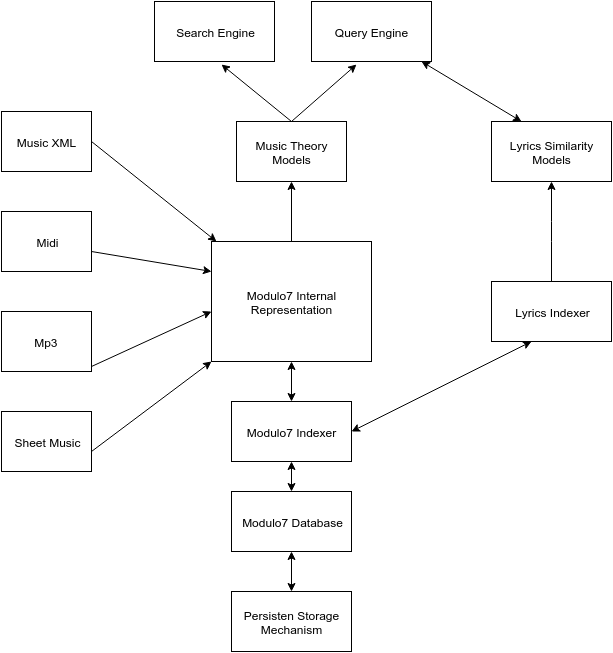
\includegraphics[width=\textwidth]{Modulo7Architecture.png}
\makeatletter
\let\@currsize\normalsize
\caption{Modulo7 architectural design}
\label{fig:figure}
\end{figure}
\newpage
\section{Client architecture}
\noindent The server exposes a sql like interface as well as a consumable API. Some sample queries would be :-
\begin{enumerate}
\item select midi files from database where $melodic\_complexity > some threshold$
\item select * from database where $artist = led\_zepplin \ and \ harmonic\_movement > harmonic\_movement(stairway\_to\_heaven)$
\item select $ num\_voices \ from \ Database \ where \ songName = someSong.midi$ 
\end{enumerate}

An API will also be exposed to the client along a remote invocation procedure. The API would primarily target single sources for specifics. Some example API would be :-
\begin{enumerate}
\item int getNumVoices(String midiFilePath)
\item double melodicContourMovement(String pngSheetFilePath)
\item double compareAverageAttack(String musicXMLFile)
\end{enumerate}

This API can be consumed for specific song analysis. As design this API will not work on a bulk of files like its sql counterpart. \\

Moreover the client also exposes a highly customized search engine based on the custom vector space representation of features extracted by Modulo7.

\section{Song sources}
\noindent At the heart of Modulo7's design is its song sources adaptors (or converters) into its own internal binary format. Each music source is a different representation and while certain sources ascribe what how music should be played (e.g musicxml, sheet music), other formats ascribe what is actually being played (e.g midi, mp3). There are many other music sources in existence (e.g guitar tablature, GUIDO format, humdrum format), but for the purposes of breadth and ubiquity, these four sources have been targeted as input for Modulo7. Note that acquiring features from each format is a domain specific challenge and inaccuracies are inherent because of that. The following subsections describe the individual formats in detail and the challenges encountered in parsing them.

\subsection{Midi format}
\noindent MIDI (short for Musical Instrument Digital Interface), is a technical specification for encoding of events on a midi enabled instrument and a protocol for interfacing and communicating between various midi enabled instruments. Typically any midi enabled electronic instrument when played, relays to its internal circuitry a message. Examples of such messages could be a particular note is being hit on a keyboard, a note is being hit off after being hit on, tempo based messages on the number of ticks per second etc. While MIDI is a technical specification for encoding music the score is being played, Modulo7 treats it as a symbolic representation of music. Midi was also a simple and popular encoding format for music and gaming industry in the nineteen ninties. \\\\
A symbolic representation is a codification of music which acts a higher level of abstraction (individual notes or chords being played) as compared to lower level representations like audio files (which codify information like waveforms). Modulo7's internal representation is also a symbolic representation. Symbolic representations are easier to manipulate when applying a music theoretic criteria. \\
Midi is one of the easier formats to parse for musical specifications. Moreover there is a big volunteer community of midi encoders. As such acquiring and parsing non trivial amounts of midi data is not a very challenging task. 

\subsection{Western Sheet Music}
Sheet music is one of the oldest forms of music in existence. Its a hand written or printed form of music that uses a specific script (a set of musical symbols on a manuscript paper) to ascribe music. Music Composers from Medieval and Modern periods of the western world use western sheet scripting to codify their work while performers play from these sources. A vast body of older work and particularly orchestral work is codified in sheet music. \\
Like midi, sheet music is also symbolic in nature. However unlike midi, its an expression of how a score should be played, rather than what is being played.  Modulo7 converts digitized versions of these sheet music (e.g sheet music stored .tiff, .png. jpeg etc formats)\\\\

A very simple example of sheet music for describing a melody is shown below. 

\begin{figure}
\centering
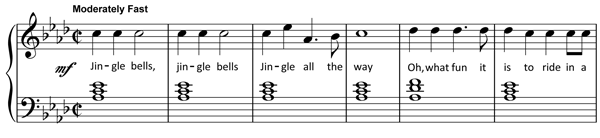
\includegraphics[width=\textwidth]{jingle-bells-sheet-music-piano.png}
\makeatletter
\let\@currsize\normalsize
\caption{Jingle bells melody sheet music representation	}
\label{fig:figure}
\end{figure}

Parsing digitized sheet music is an extremely challenging task. It requires a solid understanding on Computer Vision and even the state of the art software in existence today cant handle all scores (especially a poorly digitized formats). Given the amount of domain knowledge required, Modulo7 uses a third party library (insert TPL here). 

\subsection{Music XML format}
\noindent Music XML format is a standard open format for exchanging digital sheet music. A music XML format is unusual as its a format that is easy to parse for computers and easy for humans to understand it. MusicXML formats are heavily used by music notation applications. Music XML format is a symbolic format and can be considered a modernization of the Sheet music format. Its disadvantage however is unlike sheet music, a performer cant read the piece and play it on the spot directly. \\
Just like Western Sheet music and midi, music XML is a symbolic format as well. Music XML is also a transcription format which specifies how a score should be played. 

\subsection{MP3 format}
\noindent For the sake of completeness, Modulo7 also supports an audio format called mp3. Its an audio encoding format that uses lossy compression to encode audio data. Mp3 gives a reasonably good approximation to other digital audio formats of music storage with a significant savings in space for storage. Its one of the defacto standards of digital music compression and transfer and playback on most digital audio players. 

\section{Modulo7 Internal Representation}

\noindent Modulo7 consists of converters that convert data into Modulo7's internal representation. This representation can be thought of a document representation on which similarity measures described in Chapter 4 can be applied to. Moreover the internal representation can be thought of as an indexed meta data structure for any source of song from which relevant information can be acquired. Hence Modulo7 indexing schematic is a symbolic representation of music much like music xml and sheet music. The converters are responsible for converting different music sources to this representation format. Its important to note that depending on there source one or more of the subcomponents of the internal representation may be missing or wrong. Modulo7 indexes songs based on each of these criteria and on top of these boolean queries can be formulated. The components are broadly categorized as the following:-\\

\noindent \textbf{Song Metadata:} The metadata aspects in a song e.g. The name of the song/ the composer/performer's name, Key Signature of the Song, Meter of the Song etc. These are global properties of the song. \\

\noindent \textbf{Voices in a song:} Similar to the Voices in Music theory, Voices in Modulo7 represent the same symbolic data as is present in the sources from which the information is parsed.\\

\noindent \textbf{Lyrics of a song:} The textual representation (along with delimiters for line breaks) for the lyrics of a song. Lyrics can live independently as separate entities (if the input to Modulo7 is a text file containing the lyrics and no other information). However midi/musicxml and sheet music have optional lyrics elements present in their transcriptions and Modulo7 transcribes from those. \\\\
In most cases though lyrics exists as a separate entity from songs. In such cases, Modulo7 separately indexes lyrics. In certain datasets, the lyrics representation is different (for example the million song dataset has a representation format as a bag of words with counts of the words occuring for each format \cite{msd}). Modulo7 accomodates such formats as well.

\begin{figure}
\centering
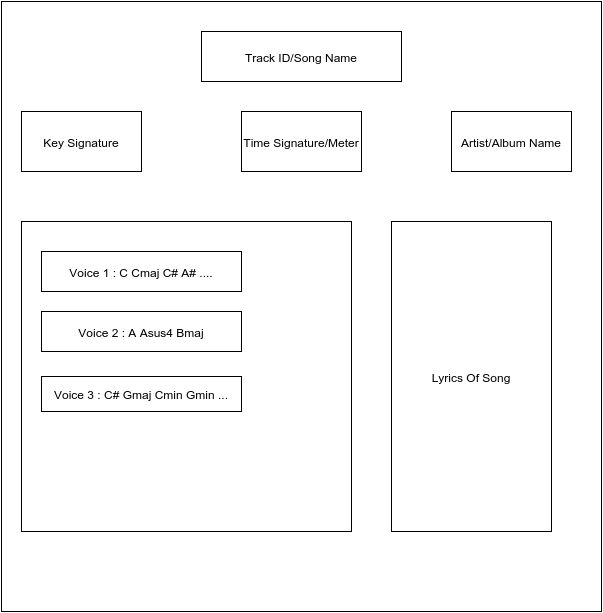
\includegraphics[width=\textwidth]{DocumentStructureOfModulo7.png}
\makeatletter
\let\@currsize\normalsize
\caption{Modulo7 internal representation}
\label{fig:figure}
\end{figure}

\section{Methodology}

\noindent This section contains the methodology followed in the information retrieval phase and then the indexing steps taken after the domain specific conversion is completed by Modulo7's adapters

\begin{enumerate}
\item Given a root directory, Modulo7 parses all the sheet music image files, mp3, midi and 
\end{enumerate}

\chapter{Experimental Evaluation}

\noindent For the purposes of evaluating Modulo7, test cases have been designed into two formats. One category of testing is micro testing, for validating correctness and precision recall for small sets of data. This ensures verifiability of algorithms and similarity measures on small datasets as well as novel explorations of data. Most MIR research is done on small scale datasets and hence falls in the purview of micro testing. The other format is macro testing which involves large datasets such as the million song dataset \cite{msd}. \\\\
A few assumptions that are made in testing are as follows :-
\begin{enumerate}
% TOD0 : Finish this section
\item In order to estimate ground truth values, the author assumed ground truth values presented in datasets used / or subjective judgements to which songs are similar to each other. These subjective judgements are procured from existing literature.
\item If the song metadata (such as keysignature, timesignature, total duration of song) is not encoded, its estimated by the parsers. This estimation id done by existing algorithms in literature. However if metadata is encoded, its assumed to be correct. 
\item Most tests are against file formats of the similar types (for example midi is tested against other symbolic files). This is due to the inherent complexity of symbolic decoding of audio formats like mp3. Also its easier to compare symbolic data against other symbolic data.
\item In the event of parsing data, there can be legal issues (e.g. the song can be copyrighted). For that reason custom parsers to build alternate research datasets (e.g the million song dataset has already derived features that Modulo7 intended to derive for Mp3 files. \cite{msd})
\item All evaluations are done against research datasets which are published in academia or exposed as public datasets in industry. 
\end{enumerate}

\section{Results of Index Compression}

\noindent The Modulo7 representation can be thought of an indexed meta data version of the song. True to all indexed data, Modulo7 represents the song in a much smaller size than the original source. The following chart demonstrates the average compression of indexed data as compared to source files on the Saarland Music Data (SMD) Dataset \cite{saarlandmsd}:-
\begin{figure}
\centering
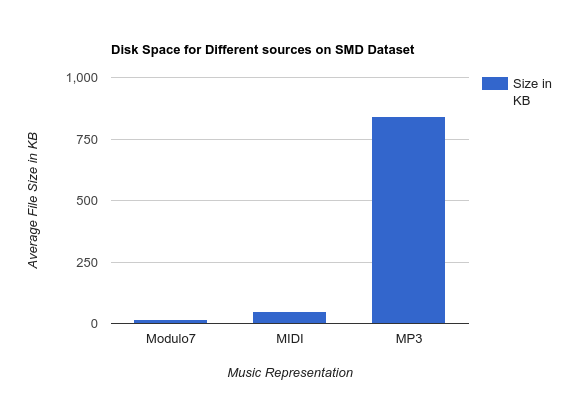
\includegraphics[width=\textwidth]{Modulo7SMDBarGraph.png}
\makeatletter
\let\@currsize\normalsize
\caption{Modulo7 architectural design}
\label{fig:figure}
\end{figure}
As expected Modulo7's serialized format expresses a song in less disk space than its source formats while keeping the symbolic information intact. The results are positive as there is a 4 time decrease in size of expressing symbolic information as compared to midi files. \\\\
A similar transformation was also done on a direct downloadable subset of the wikifonia dataset in order to compare Modulo7 internal representation against normal 

\section{Result on Memory and Disk space \\ usage}

\noindent In order to compare the memory and disk space requirements, Modulo7 was tested against its closest competitor jMIR's \cite{jMIR} jSymbolic component. Both frameworks are written in Java and both involve extraction of features. However jMIR is more exhaustive in what features it extracts so only a subset of those that are also extracted by Modulo7 are considered. 

\section{Results on similarity measures}

\noindent This set of experiments determine the precision and recall values for the similarities defined in \ref{similarity} on ground truth data extracted from \cite{msd}. Modulo7 does not claim to improve on the state of the art when it comes to similarity metrics. However the following tests are carried out : 

\begin{enumerate}
\item Benchmarks are done against the SIMILIE software stack \cite{similie} after taking into account the inherent speed difference between R\cite{similietechnicalmanual} and Java for specific melodies
\item The state of the art similarity measures for melodies are generalized to polyphonic music and tested against newer datasets as compared to \cite{msd} to ascertain recall and precision values
\item 
\end{enumerate}  

\section{Results on KK Tonality Profiles algorithm}

\noindent In order to test the KK Tonality algorithm given in \ref{kktonality}, Modulo7 is benchmarked against a big subset of the Wikifonia data set of lead sheets in the compact mxl format (variant of the music xml format) \cite{WikifoniaDataset}. The original dataset of the Wikifonia is now no longer available but a sizable subset of 6715 songs are currently downloadable and copyright free. Out of this set, 1314 have key signatures embedded in the song sources. The experiment involves comparing the key signatures embedded inside the key signatures versus the implied key signatures the KK Tonality estimates from the pitch histogram of the songs parsed from this source. A special MXL parser (a minor variant of the music xml parser) was developed for this purpose. The scoring scheme for this experiment was simple, if the key signature was correctly identified then score of 1 otherwise score of 0. In this particular dataset, key signatures are partially known (\textbf{since the number of sharps or flats in the key signatures are always encoded in music xml files} so only relative major/minor are needed to be ascertained). As a consequence only two choices are to be made between key signatures for each file giving a baseline of 50 percent. In this particular example, KK Tonality's performance is how well it can distinguish between relative minors and majors. \\\\
After running the KK Tonality algorithm on the wikifonia dataset, 1129 out the total 1314 key signatures are correctly identified leading to an accuracy of \text{85.9 percent}. This is commensurate with the reported accuracies in \cite{kkTonalityKeyFinding}.


\section{Results on lyrics similarity and statistics analysis}

\noindent On top of the experiments done for Song sources incorporating tonal information, there were specific experiments that were carried out for 

\appendix
\addcontentsline{toc}{chapter}{APPENDICES}
\chapter{Third Party Libraries Used}

\noindent Modulo7 is a significant software engineering effort. This is partly due to the fact that Modulo7 tends to address speed related issues that are prevalent in other frameworks and partly due to the disparate sources of music that it supports. As such Modulo7 utilizes a number of third party libraries in its operations. These libraries and their roles are mentioned below:-

\section{Apache Lucene}

\noindent Apache Lucene is a full text search engine library written in Java. Apache Lucene is used for indexing text documents, spelling correction and other such functionality. \\
In context of Modulo7, Apache Lucene is used to maintain inverted indices of lyrics either independently acquired from text files containing lyrics or from emdedded lyrics in the Modulo7 supported sources. 

\section{Apache Avro}

\noindent Apache Avro is a serialization library used to store Modulo7 objects to disk. This allows for faster retrieval of parsed objects instead of having to reparse entire song sources again and again.

\section{Echo Nest jEN API}

\noindent The toughest challenge in all of Modulo7 was to parse symbolic information from audio sources. In order to accomplish this, Modulo7 relied on the Echo Nest's client library to convert mp3 files into chromagram representation of music \cite{chromagramtutorial}. The chromagram representation is acquired directly by converting mp3 representation into the frequency domain by Echo Nest. Modulo7 treats this process as a black box, as it is interested in finding out only the chromagram representation (from which identifying notes and chords become much simpler). 

\section{Antlr}

\noindent Antlr (Another language recognition tool) is a framework used to develop lexers and parses for custom programming languages. In case of Modulo7, Antlr was used to develop the Modulo7SQL Custom query language.

\section{Jsoup}

\noindent Jsoup is a library used for parsing XML documents written in Java. In case of Modulo7, Jsoup is used to parse music xml documents and present song representations to the Modulo7 engine. 

\section{Audiveris}

\noindent Audiveris is a OMR (Optical Music Recognition System) written in Java which converts digitized sheet music files into musicxml files. Audiveris is used to parse sheet music files into Modulo7 song representations.

\section{Alchemy} \label{Alchemy}

\noindent Alchemy is an implementation of NLP(In general AI) as a service model by IBM. Alchemy provides support for language ID, semantic analysis of arbitrary documents and text. In Modulo7, Alchemy is used for analyzing lyrics.  

\section{Apache JCS (Java Caching System)}

\noindent Apache JCS is used as a distributed in memory cache to cache the results of Modulo7 custom queries and similarity results for the queries made in the past. 

\chapter{Algorithms in use in Modulo7}

\noindent There are certain algorithms in literature that are directly implemented in Modulo7. These algorithms facilitate the smooth functioning of Modulo7's indexing in face of incomplete metadata. Some notable algorithms that have been used are briefly described in the following subsections

\section{KK Tonality Profiles and a Key Estimation Algorithm} \label{kktonality}

\noindent Many music sources have the key signature inscribed in it. For example a midi file might have the key signature bytes transcribed. In the event that this information is not present, it must be inferred from the recording. This is required for certain similarity measures that need the key signature of the song for preprocessing steps  in particular for tonality alignment (\ref{sim:unequal}). There are many methods for achieving this including non trivial tree representations of polyphonic music to estimate key \cite{treemodel}. However in Modulo7, the author has implemented a simpler model for tonality estimation based on templates called KK tonality profiles \cite{kkTonalityKeyFinding} \\

\noindent The premise of the KK tonality profile stems from experiments done in \cite{kkTonalityKeyFinding} and \cite{kkcognitive} which estimate how likely a user is to ascribe a note to a series on notes played on a melody or an incomplete harmonic element in different keys. The notes guessed correlate to the relative prominence of a note in a given key(what this the frequency and total duration a note is played in a song in a given key). After many experiments, the experimenters collected the aggregate duration for each note for each key. This experiment was  repeated for all 12 major and 12 minor keys. They were able to acquire 24 profiles (vectors of real numbers) which represent a quantitative measure of the key. For example the profiles for C Major and C Minor are respectively \cite{kkcognitive}.
\begin{equation} \label{kkprofiles}
\begin{aligned}
  CMajor = <6.35, 2.23, 3.48, 2.33, 4.38, 4.09, 2.52, 5.19, 2.39, 3.66, 2.29, 2.88> \\
  CMinor = <6.33, 2.68, 3.52, 5.38, 2.60, 3.53, 2.54, 4.75, 3.98, 2.69, 3.34, 3.17>, 
\end{aligned}
\end{equation}

\noindent The profiles of the other keys can be achieved by rotating the vector by the intervalic distance of the root notes of the key and root note their reference Key(CMajor for major keys and CMinor for minor keys). \\

\noindent The key estimation algorithm leverages the kk tonality profiles as input. The algorithm is as follows:-

\begin{algorithm}

\label{CHalgorithm}
\begin{algorithmic}[1]
\Procedure{Predict Key Signature(song)} {}
\State Define CMaj and CMin as per eqn \ref{kkprofiles}
\State Define MajProf and MinProf = [] % empty sets
\State MajProf.add(CMaj) and MinProf.add(CMin)
\State Define prev\_Key = C 
\For {key in western keys [D to B]}
\State MajProf[key] = left\_shift(MajProf[prev\_Key])
\State MinProf[key] = left\_shift(MinProf[prev\_Key])
\State prev\_Key = key
\EndFor
\State song\_Pitch\_Hist = compute\_song\_tonal\_histogram(song) as per \ref{NPDH}
\State best\_Key = CMin, best\_Corr = $-\infty$
\For {key, maj\_prof in MajProf}:
\If {correlation(maj\_prof, song\_Pitch\_Hist) > best\_Corr}
\State best\_Key = key
\State best\_Corr = correlation(maj\_prof, song\_Pitch\_Hist)
\EndIf
\EndFor
\For {key, mij\_prof in MijProf}:
\If {correlation(min\_prof, song\_Pitch\_Hist) > best\_Corr}
\State best\_Key = key
\State best\_Corr = correlation(min\_prof, song\_Pitch\_Hist)
\EndIf
\EndFor
\Return best\_Key
\EndProcedure
\end{algorithmic}
\end{algorithm}

\subsection{Chord Identification from Chromagram}

\noindent A chromagram \cite{chromagramtutorial} is a representation of a song in frequency domain with relative intensities of notes in a short window frames of analysis in songs. This chromagram representation is central to acquiring symbolic description from audio sources. Once a chromagram is acquired, ascertaining chords in it becomes important(in particular because harmonic elements are non trivial to ascertain in a given chromagram). Modulo7 implements an algorithm described in \cite{chord-detection} in order to detect chords in chromagrams. This procedure is based on chromagram templates of different chords and correlation of current chromagram with these templates.


%% REFERENCES

% if you use BIBTEX
\bibliographystyle{IEEEtran}
\bibliography{thesis}

\end{document}